\Subhead{1.1.2}{Силовое воздействие на линейные и слабонелинейные колебательные системы}
\textbf{Механизм.} Внешняя сила $F_0\cos\Omega t$ непосредственно сообщает энергию: мгновенная мощность $F\dot x$. Около резонанса сила действует в такт со скоростью. Установившийся ответ существует, когда средний приток компенсирует потери.

Подставим $x=\operatorname{Re}(X\e^{-\ii\Omega t})$ в \eqref{eq:linear}. При $f=F_0/m$
\begin{equation}\label{eq:chi}
 X=\frac{f}{\omega_0^2-\Omega^2-2\ii\gamma\Omega},\qquad
 A=\frac{f}{\sqrt{(\omega_0^2-\Omega^2)^2+4\gamma^2\Omega^2}}.
\end{equation}
В записи $x=A\cos(\Omega t-\varphi)$ фаза запаздывает: от $0$ при низкой частоте через $\pi/2$ при $\Omega=\omega_0$ до $\pi$ при высокой. В резонансе скорость совпадает по фазе с силой и
\begin{equation}
 \avg P=\tfrac12F_0A\Omega\sin\varphi=m\gamma\Omega^2A^2.
\end{equation}
При $Q\gg1$: $A(\omega_0)=QF_0/k$, полная ширина по половине мощности $\Delta\Omega\simeq2\gamma=\omega_0/Q$, время установления амплитуды $\tau_A=1/\gamma$. Точный максимум смещения расположен при $\Omega_r=\sqrt{\omega_0^2-2\gamma^2}$, если этот корень существует; максимум поглощаемой мощности при постоянном $F_0$ --- при $\omega_0$. При $\gamma=0$ на точном резонансе конечного стационарного ответа нет: $x\sim ft\sin\omega_0t/(2\omega_0)$.
\begin{center}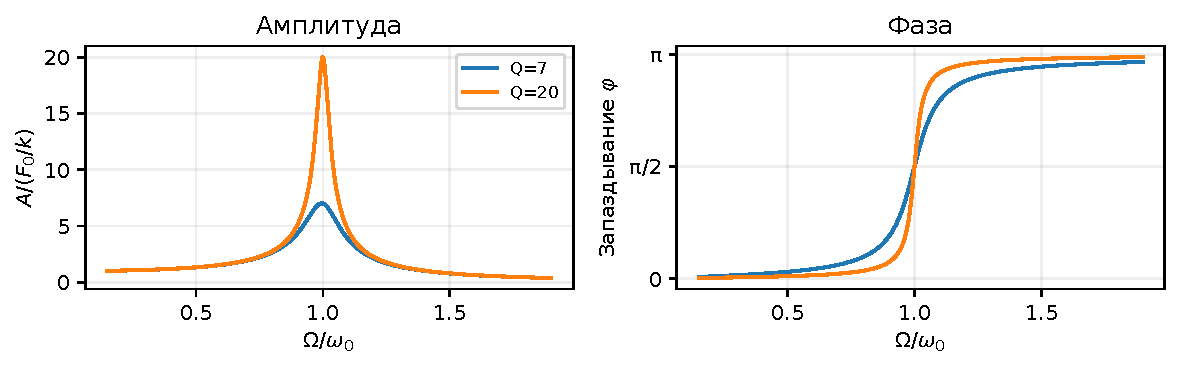
\includegraphics[width=.83\linewidth]{figures/linear_response.pdf}\end{center}

\paragraph{Поправка слабой нелинейности.}
В модели Дуффинга
\begin{equation}\label{eq:duffing}
 \ddot x+2\gamma\dot x+\omega_0^2x+\alpha x^3=f\cos\Omega t
\end{equation}
предполагается $|\alpha|A^2\ll\omega_0^2$. Первая гармоника $x^3$ равна $3A^3\cos(\Omega t-\varphi)/4$. Поэтому
\begin{equation}\label{eq:duffingresponse}
 f^2=A^2[(\omega_0^2-\Omega^2+3\alpha A^2/4)^2+4\gamma^2\Omega^2],
 \qquad \omega(A)\simeq\omega_0+\frac{3\alpha A^2}{8\omega_0}.
\end{equation}
Жёсткая нелинейность ($\alpha>0$) наклоняет резонанс вправо, мягкая --- влево. При достаточном изгибе появляются две устойчивые амплитуды, разделённые неустойчивой ветвью. При медленной перестройке наблюдаются скачки и гистерезис. Это пример \emph{слабонелинейного силового воздействия}; исследование всех бифуркаций Дуффинга для данного вопроса не требуется. Устойчивость ветвей определяется динамикой, а не одним числом корней алгебраического баланса.
\begin{center}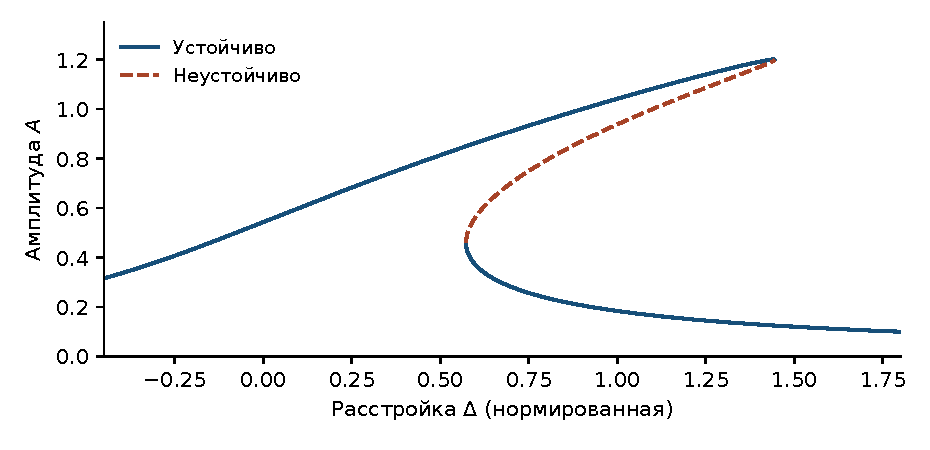
\includegraphics[width=.66\linewidth]{figures/duffing.pdf}\end{center}
% Самостоятельная проверка: проекция кубической силы на первую гармонику.
